\documentclass[10pt, oneside]{article}
\usepackage[a4paper, total={5.5in, 9in}]{geometry}
\usepackage[ngerman]{babel}

\usepackage{blindtext}
\usepackage{titlesec}
\usepackage{amsmath}
\usepackage[hidelinks]{hyperref}
\usepackage{parskip}
\usepackage{graphicx}
\usepackage{longtable}
\usepackage[shortlabels]{enumitem}
\usepackage{multirow}
\usepackage{nccmath}
\usepackage{rotating}
\usepackage{makecell}
\usepackage{multicol}
\usepackage{capt-of}
\usepackage{csquotes}
\usepackage{amsfonts}
\usepackage{caption}

\captionsetup[table]{position=bottom}

\titleformat{\section}
    {\normalfont\Large\bfseries}{}{0pt}{}

\let\oldsection\section
\renewcommand{\section}{
  \renewcommand{\theequation}{\thesection.\arabic{equation}}
  \oldsection}
\let\oldsubsection\subsection
\renewcommand{\subsection}{
  \renewcommand{\theequation}{\thesubsection.\arabic{equation}}
  \oldsubsection}

\makeatletter
\renewcommand{\maketitle}{
    \bgroup
    \centering
    \par\LARGE\@title  \\[20pt]
    \par\large\@author \\[10pt]
    \par\large\@date
    \par
    \egroup
}
\makeatother


\title{Mathematische Grundlagen\\[5pt]\Large WiSe 2024/25\\[10pt]\Large L{\"o}sungen zu den Aufgaben 13, 16, 24, 26}
\author{Volodymyr But}
\date{}

% - - - - - - - - - - - - - - - - - - - - - - - - - - - - - - - - - - - - - - %

\begin{document}
\sloppy

\maketitle
\vspace{25px}

\section{Aufgabe 13}

Es seien $X = Y = \{1, 2, 3, 4 ,5\}$ und $f : X \longrightarrow Y$ definiert durch

\begin{equation*}
    f(k) :=
    \begin{cases}
        k + 1,& \text{ falls } k \leq 4 \\
        1,    & \text{ falls } k =    5
    \end{cases}
\end{equation*}

\begin{enumerate}[(a)]
    \item Skizzieren Sie den Graph von $f$.
        \vspace{15pt}
        \begin{figure*}[h]
            \centering
            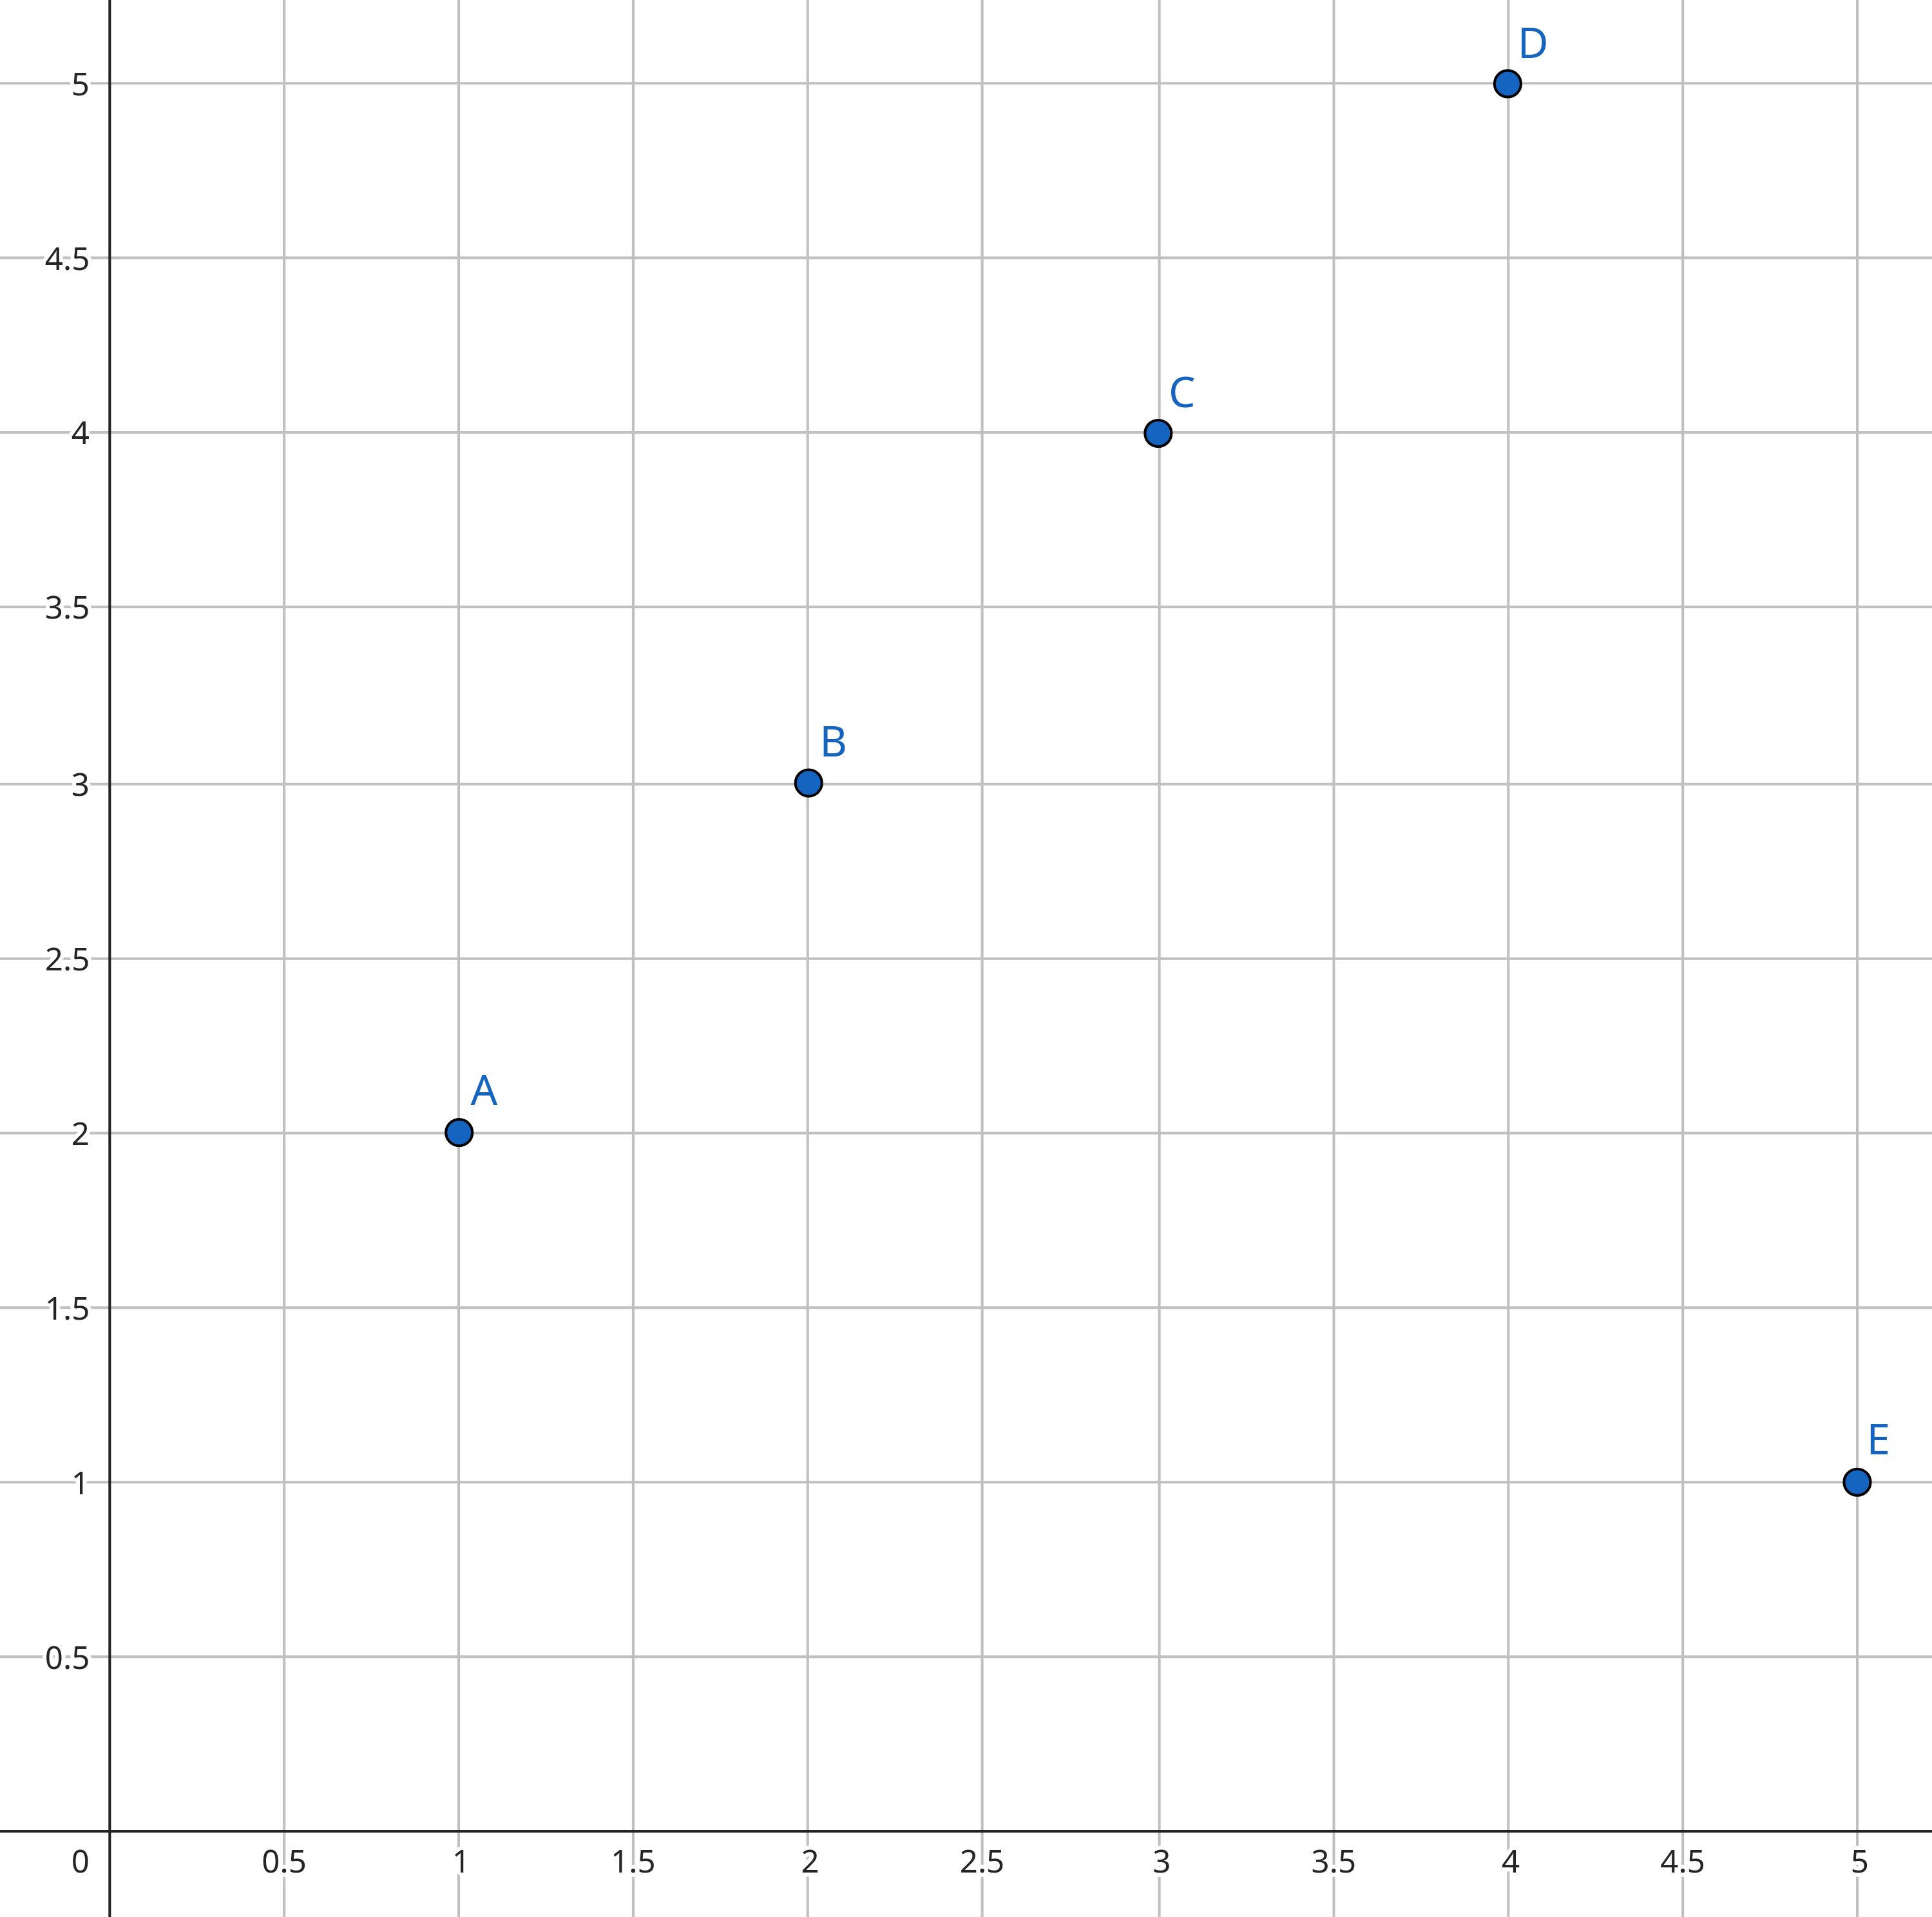
\includegraphics{./assets/13-01.png}
        \end{figure*}

    \item Bestimmen Sie die Urbilder $f^{-1}(A)$, $f^{-1}(B)$, wobei $A := \{1,4\}$
        und $B := \{2,5\}$.

        \begin{equation*}
            \begin{aligned}
                f^{-1}(\{1, 4\}) &= \{x \in X : f(x) \in \{1, 4\}\} = \{3, 5\} \\[5pt]
                f^{-1}(\{2, 5\}) &= \{x \in X : f(x) \in \{2, 5\}\} = \{1, 4\}
            \end{aligned}
        \end{equation*}

\end{enumerate}

\pagebreak
\section{Aufgabe 16}
\setcounter{section}{16}

Es sei $f : \mathbb{R} \rightarrow \mathbb{R}$, $f(x) = x^3 + ax$, $a \in \mathbb{R}$.

\begin{enumerate}[(a)]
    \item Skizzieren Sie jeweils den Graph von $f$ f"ur $a = 1$ und $a = -2$.

        \begin{figure}[h]
            \centering
            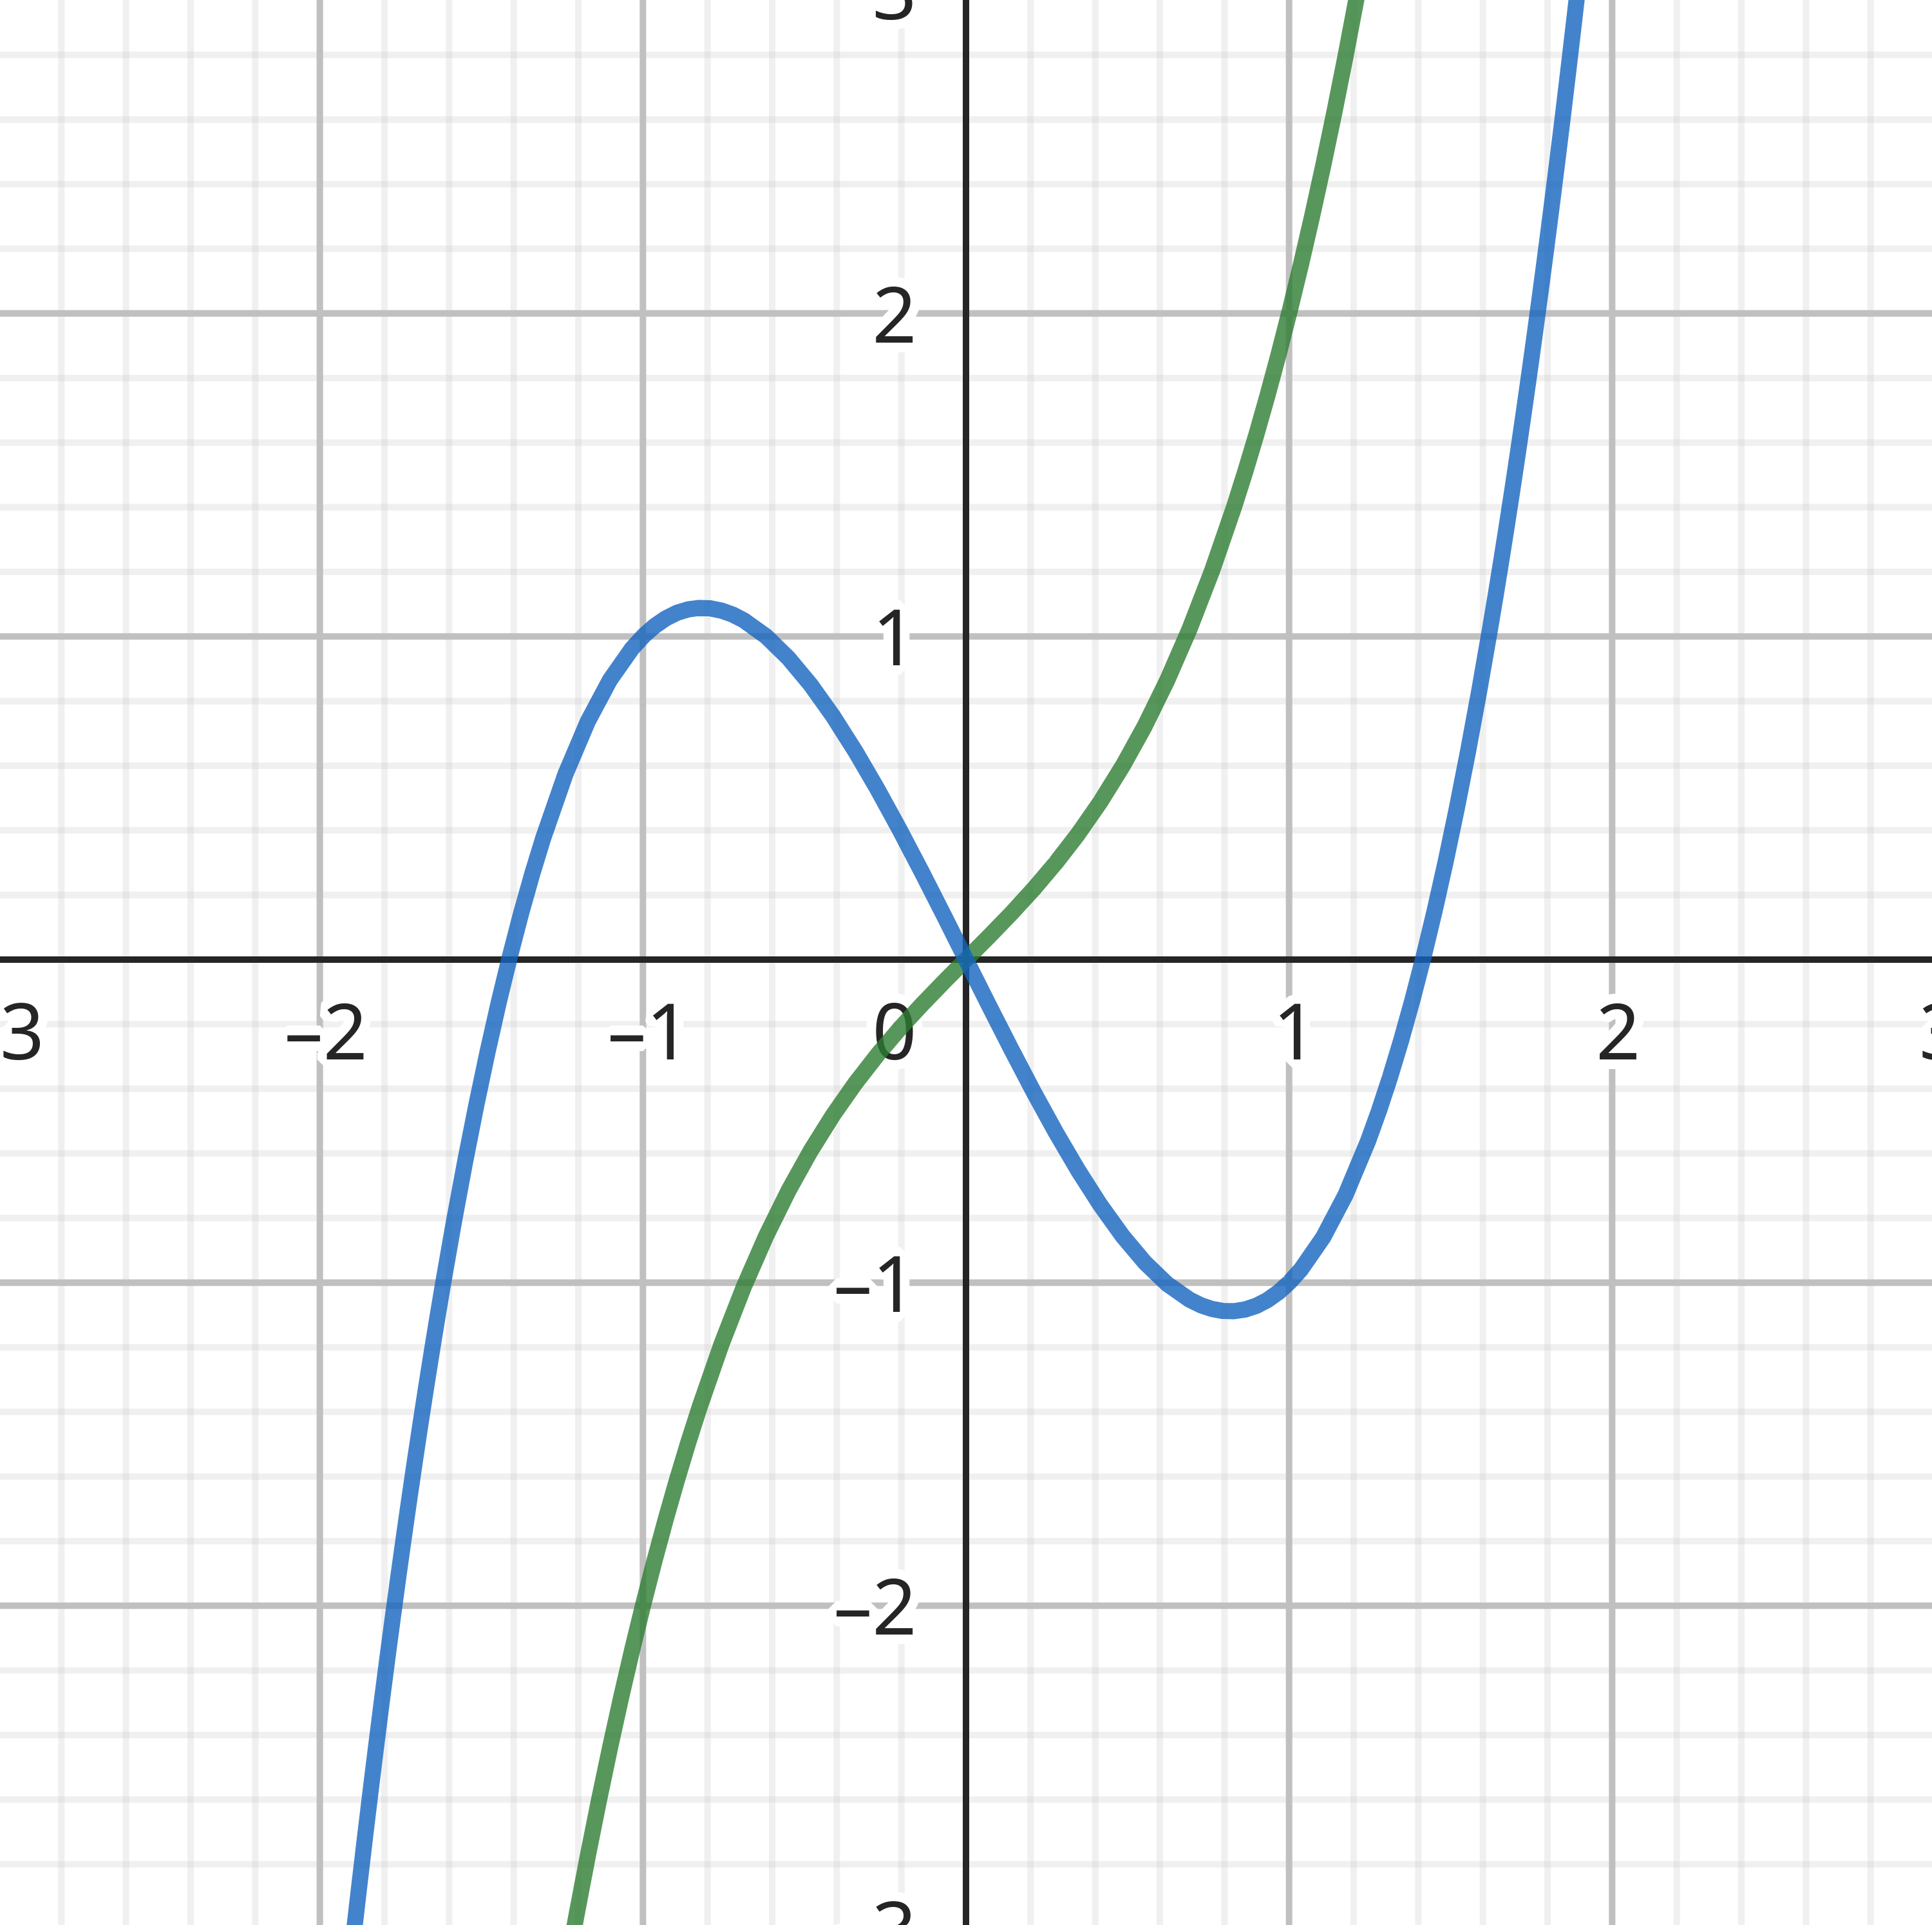
\includegraphics{./assets/16-a.png}
        \end{figure}

    \item Zeigen Sie, dass f"ur $a < 0$ die Abbildung $f$ nicht injektiv ist.

        \textbf{Beweis}. Eine Funktion ist $f$ injektiv, wenn
        \begin{equation*}
            \forall x_1, x_2 \in X, x_1 \neq x_2 \implies f(x_1) \neq f(x_2)
        \end{equation*}
        Um zu zeigen, dass $f$ nicht injektiv ist, gen"ugt es daher zu zeigen,
        dass
        \begin{equation*}
            \exists x_1, x_2 \in X, x_1 \neq x_2 \implies f(x_1) = f(x_2)
        \end{equation*}
        Setzen wir $f(x_1) = f(x_2)$, so erhalten wir:
        \begin{equation*}
            \begin{array}{rcl}
                x_1^3 + ax_1 &=& x_2^3 + ax_2 \\[5pt]
                x_1^3 - x_2^3 &=& -a(x_1 - x_2)  \\[10pt]
                \dfrac{x_1^3 - x_2^3}{x_1 - x_2} &=& -a
            \end{array}
        \end{equation*}
        Als N"achstes zeigen wir, dass
        \begin{equation*}
            \forall x_1,x_2 \in X, x_1 \neq x_2 \implies \dfrac{x_1^3 - x_2^3}{x_1 - x_2} > 0
        \end{equation*}
        Dies lässt sich wie folgt darstellen:
        \begin{equation*}
            \begin{aligned}
                      &(((x_1^3 - x_2^3) > 0) \land ((x_1 - x_2) > 0))\  \lor \\
                \lor\ &(((x_1^3 - x_2^3) < 0) \land ((x_1 - x_2) < 0)) \\
                \iff  &(((\sqrt[3]{x_1^3} - \sqrt[3]{x_2^3}) > \sqrt[3]{0}) \land ((x_1 - x_2) > 0))\ \lor \\
                \lor\ &(((\sqrt[3]{x_1^3} - \sqrt[3]{x_2^3}) < \sqrt[3]{0}) \land ((x_1 - x_2) < 0)) \\
                \iff  &(((x_1 - x_2) > 0) \land ((x_1 - x_2) > 0))\ \lor \\
                \lor\ &(((x_1 - x_2) < 0) \land ((x_1 - x_2) < 0)) \\
                \iff  &((x_1 - x_2) > 0)\ \lor\ ((x_1 - x_2) < 0) \\
                \iff  &(x_1 > x_2)\ \lor\ (x_1 < x_2) \\
                \iff  &x_1 \neq x_2 \quad \text{\underline{q.e.d.}}
            \end{aligned}
        \end{equation*}
        Und weil
        \begin{equation*}
            \dfrac{x_1^3 - x_2^3}{x_1 - x_2} > 0 \quad\text{und}\quad \dfrac{x_1^3 - x_2^3}{x_1 - x_2} = -a
        \end{equation*}
        muss $a < 0$ sein, um $f(x_1) = f(x_2)$ f"ur $x_1 \neq x_2$ zu erf"ullen.
        \begin{center}
            \underline{q.e.d.}
        \end{center}
\end{enumerate}

\section{Aufgabe 24}

Es seien $f : X \rightarrow Y$ eine Abbildung und $A, B \subset Y$. Zeigen Sie,
dass folgendes gilt:
\begin{equation*}
    \begin{gathered}
        f^{-1}(A \cap B) = f^{-1}(A) \cap f^{-1}(B)\text{,}\\
        f^{-1}(A \cup B) = f^{-1}(A) \cup f^{-1}(B)
    \end{gathered}
\end{equation*}

\begin{equation*}
    \begin{aligned}
        f^{-1}(A \cap B) &= \{x \in X : f(x) \in \{A \cap B\}\} = \\
                         &= \{x \in X : f(x) \in A \text{ und } f(x) \in B\} = \\
                         &= \{x \in X : f(x) \in A\} \cap \{x \in X : f(x) \in B\} = \\
                         &= f^{-1}(A) \cap f^{-1}(B) \quad \text{\underline{q.e.d.}}
    \end{aligned}
\end{equation*}

\begin{equation*}
    \begin{aligned}
        f^{-1}(A \cup B) &= \{x \in X : f(x) \in \{A \cup B\}\} = \\
                         &= \{x \in X : f(x) \in A \text{ oder } f(x) \in B\} = \\
                         &= \{x \in X : f(x) \in A\} \cup \{x \in X : f(x) \in B\} = \\
                         &= f^{-1}(A) \cup f^{-1}(B) \quad \text{\underline{q.e.d.}}
    \end{aligned}
\end{equation*}

\section{Aufgabe 26}

Untersuchen Sie folgende Abbildungen auf Injektivität

\begin{enumerate}[(a)]
    \item $f : \mathbb{R} \rightarrow \mathbb{R}$, $f(x) = x^4 - 1$,

        \begin{equation*}
            \begin{array}{rcl}
                f(x_1) &=& f(x_2) \quad (x_1 \neq x_2) \\[5pt]
                x_1^4 - 1 &=& x_2^4 - 1 \\[5pt]
                x_1^4 &=& x_2^4 \\[5pt]
                |x_1| &=& |x_2| \quad \text{\underline{q.e.d.}}
            \end{array}
        \end{equation*}

    \item $f : \mathbb{N} \rightarrow \mathbb{R}$, $f(x) = 4x^2$,

        \begin{equation*}
            \begin{array}{rcl}
                f(x_1) &=& f(x_2) \quad (x > 0, x_1 \neq x_2) \\[5pt]
                4x_1^2 &=& 4x_2^2 \\[5pt]
                x_1^2 &=& x_2^2 \implies \emptyset
            \end{array}
        \end{equation*}

    \pagebreak
    \item $f : \mathbb{R} \setminus \{2\} \rightarrow \mathbb{R}$, $f(x) = \dfrac{3}{(2 - x)^2}$.

        \begin{equation*}
            \begin{array}{rcl}
                f(x_1) &=& f(x_2) \quad (x \neq 2, x_1 \neq x_2) \\[5pt]
                \dfrac{3}{(2 - x_1)^2} &=& \dfrac{3}{(2 - x_2)^2} \\[10pt]
                (2 - x_1)^2 &=& (2 - x_2)^2 \\[5pt]
                |2 - x_1| &=& |2 - x_2| \\[5pt]
                |x_1| &=& |x_2| \quad \text{\underline{q.e.d.}}
            \end{array}
        \end{equation*}

\end{enumerate}

\end{document}
